%
%\boxx{\subsubsection{Some Sources for Market Failure}
%	\itex{
%		\item 
%		\item Imperfect competition (see \ref{sec:monopoly})
%		\item External effects (see \ref{sec:externaleffects})
%		\item Public goods (see \ref{sec:publicgoods})
%		\item Imperfect information (see \ref{sec:imperfectinformation})
%		\item Imperfect rational behavior (see \ref{sec:behavioraleconomics})
%		\item Macroeconomic disturbances (e.g., unemployment)
%	}
%}




\pbn
\section{When market are not free: Price controls}\label{sec:pricecontrols}
\subsection{Maximum price}

A legal maximum price, set to protect consumers, establishes an upper limit for the sale of a good. One example is the price fixing in rental apartments. It is ineffective if set above the equilibrium price, as depicted in \autoref{fig:maxprice}; it becomes binding when placed below the equilibrium price, as shown in \autoref{fig:maxprice-binding}. This can lead to a deadweight loss due to missed mutually beneficial transactions.

\begin{figure}\centering
	\includegraphics[width=.6\linewidth]{../../../pic/maxprice-nonbinding}
	\caption{Non binding maximum price}\label{fig:maxprice}
\end{figure}
\pbn

\begin{figure}\centering
	\includegraphics[width=.7\linewidth]{../../../pic/maxprice-binding}
	\caption{Binding maximum price}\label{fig:maxprice-binding}
\end{figure}

\subsection{Minimum price}

A legal minimum price is a rule that sets the lowest price for a product, protecting sellers. For example, minimum wage protect the seller of labor time. Only when this minimum price is higher than the normal price, it is binding and affects the market. 

\exex{Welfare and price controls}{
	Analyze the two scenarios above. Can you sketch in both plots consumer and producer surplus. Who is better off? Who is worse off? And, does overall welfare increase or decrease?
}

\subsection{Taxes}

Taxes change how things are bought and sold. When there's a tax, people who buy things pay more, and people who sell things get less money, no matter who the tax is on. Tax incidence shows how the burden of the tax is divided between buyers and sellers, see \autoref{fig:Taxesofbuyers} and \autoref{fig:Taxesofsellers}.

\pbn
The tax has several effects:
\itex{
	\item Quantity of goods sold decreases.
	\item Sales decrease after the tax is applied.
	\item The tax burden is shared between buyers and sellers, no matter who the tax is imposed on.
	\item There is a loss of welfare (deadweight loss).
}

\pbn

\begin{figure}
	\includegraphics[width=.7\linewidth]{../../../pic/micro/taxesbad}
	\caption{Taxes of buyers}\label{fig:Taxesofbuyers}
\end{figure}


\pbn
\exex{Tax Consumer}{
	%	\begin{minipage}{0.5\textwidth}
		The figure here illustrates the consequences of an fixed excise tax and its implied dead-weight loss when the producers have to pay the tax. (An excise tax is a tax imposed by the government that applies when a producer makes a sale. A fixed excise tax is an amount that the seller must return to the government for each unit sold to a customer.)
		%	\end{minipage}
	\begin{center}
		\includegraphics[width=.6\linewidth]{../../../pic/micro/taxsupply}\captionof{figure}{Welfare implications of a tex}
	\end{center}
	
	Sketch a similar figure\dots
	\abcx{
		\item \dots when the consumer have to pay the tax.
		\item \dots when there is a price ceiling. (A price ceiling describes a market where exchanges are not permitted above
		a certain price.)
		\item \dots when there is a price floor. (A price floor describes a market where exchanges are not permitted under a certain price.)
	}
}



\pbn

\begin{figure}
	\includegraphics[width=.7\linewidth]{../../../pic/micro/taxesbad2}
	\caption{Taxes of sellers}\label{fig:Taxesofsellers}
\end{figure}




\exex{Laffer curve}{
	The Laffer Curve is an economic concept that illustrates the relationship between tax rates and tax revenue. It is named after economist Arthur Laffer who sketched that curve in 1974 on a napkin (see \autoref{fig:napkin}) talking to Dick Cheney and Donald Rumsfeld, two former important US politicians. The curve suggests that there exists a tax rate that maximizes government revenue. At very low and very high tax rates, the government revenue generated may be relatively low, as taxpayers either have little incentive to work (at very high rates) or can evade taxes (at very low rates).
	
	\begin{center}
		\centering
		\includegraphics[width=0.7\linewidth]{../../../pic/napkin}
		\captionof{figure}{Laffer's napkin
			\label{fig:napkin}}
		\note{Source: National Museum of American History, see: \url{https://americanhistory.si.edu/collections/search/object/nmah_1439217}.}
	\end{center}
	
	Now, visit \url{https://www.online-vwl.de/english/micro/dynvwlengsu3.html} and consider the interactive graph. You can change the tax rate and draw the Laffer curve. What is the impact of the supply and demand elasticity? Can you always spot consumer surplus, producer surplus, tax revenue, and deadweight loss.
}

\pbn
\subsection{Subsidies}
Subsidies are like negative taxes, producing the opposite impacts of taxes, that are:
\itex{
	\item More quantity being bought and sold, respectively.
	\item A boost in total sales due to the subsidy.
	\item The benefit are shared between buyers and sellers, regardless of who receives the subsidy.
}

\pbn
\exex{Exercise: Minimum Wage}{
	Analyze welfare effects of a minimum wage that is above the market clearing equilibrium wage.
}

\pbn
\exex{Social Surplus}{
	\pencilbig The demand and supply functions in a competitive market are given
	by
	$$p = 20 - \frac{1}{2}q$$
	and
	$$p = 5 + q$$
	\abcx{\item What is the equilibrium quantity in this market?
		\item  What is the equilibrium price in this market?
		\item  If the price was 10\% higher than the market equilibrium, what would	be the excess supply?
		\item  If the price was 20\% lower than the market equilibrium, what would be the amount of shortage?
		\item  What is the consumers' surplus in this market?
		\item  What is the social surplus in this market?
	}
}

\pbn
\solx{Social Surplus}{
	\abcx{\item 10
		\item 15
		\item 4.5
		\item 9
		\item 25
		\item 75	
	}
}

\pbn
\exex{Markets Are Connected}{
	\readbig Read section 11.1 of \cite{Emerson2020Intermediate} which is freely available, see: \url{https://open.oregonstate.education/intermediatemicroeconomics/chapter/module-11/} and answer the following problem.\\
	\pencilbig
	Consider the following goods: gasoline powered cars (\textit{cars}), electricity powered cars (\textit{e-cars}), and gasoline (\textit{gas}).
	
	\abcx{\item Are the goods \textit{cars} and \textit{gas} more likely to be substitutes or complements? Explain your decision.
		\item Indicate whether the following pairs of goods are more likely to be substitutes or complements: (1) cars and e-cars (2) e-cars and gas.
		\item  Suppose a new, easy accessible, and huge oil field is found. As a consequence, you expect that the price for gasoline will fall. In the following, you should analyze the impact of this exogenous shock on the three markets in further detail. Assume thereby that the price of gasoline does not alter production of \textit{cars} and \textit{e-cars}, respectively. The three plots below represent the three markets where the supply function, $S$, and demand functions, $D$, refer to the market circumstances before the exogenous shock has happened.\\
		Sketch in the three plots---for each market---shifts of the supply function and/or the demand function that may happen due to the exogenous shock. Discuss the new the equilibrium prices and quantities on the respective markets.
		
		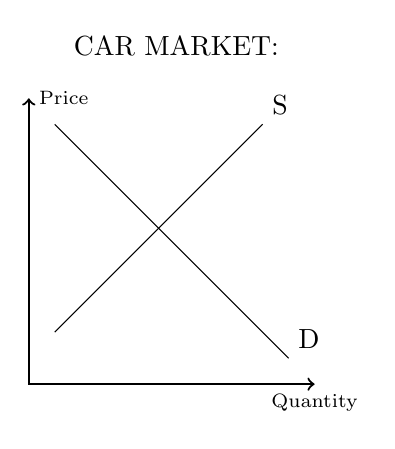
\begin{tikzpicture}[scale=.33]
			%	\draw [color=gray!50,opacity=0.5]  [step=10mm] (0,0) grid (10,10);
			%HOME	
			\draw[thick,<->] (0,11) node[right,font=\scriptsize]{Price}--(0,0)--(11,0) node[below,font=\scriptsize]{Quantity}; 
			\draw (1,10) -- (10,1) node[above right] {D};
			\draw (1,2) -- (9,10) node[above right] {S};
			\draw[] (10,13) node[left]{CAR MARKET:};
			%\draw[thick, red] (0,2) node[left]{$P^W$} -- (10,2)  ;
		\end{tikzpicture}
		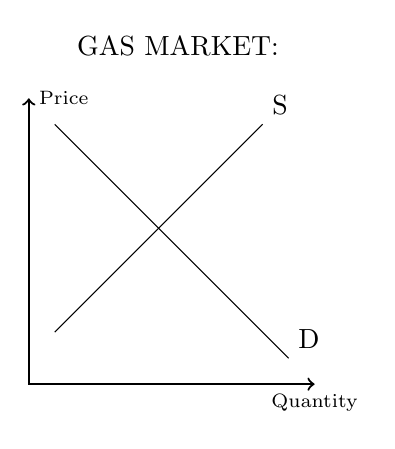
\begin{tikzpicture}[scale=.33]
			%	\draw [color=gray!50,opacity=0.5]  [step=10mm] (0,0) grid (10,10);
			%HOME	
			\draw[thick,<->] (0,11) node[right,font=\scriptsize]{Price}--(0,0)--(11,0) node[below,font=\scriptsize]{Quantity}; 
			\draw (1,10) -- (10,1) node[above right] {D};
			\draw (1,2) -- (9,10) node[above right] {S};
			\draw[] (10,13) node[left]{GAS MARKET:};
			%\draw[thick, red] (0,2) node[left]{$P^W$} -- (10,2)  ;
		\end{tikzpicture}
		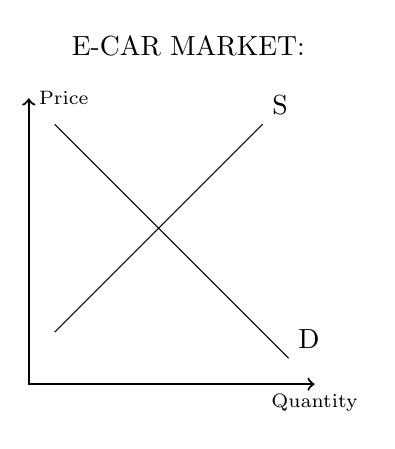
\begin{tikzpicture}[scale=.33]
			%	\draw [color=gray!50,opacity=0.5]  [step=10mm] (0,0) grid (10,10);
			%HOME	
			\draw[thick,<->] (0,11) node[right,font=\scriptsize]{Price}--(0,0)--(11,0) node[below,font=\scriptsize]{Quantity}; 
			\draw (1,10) -- (10,1) node[above right] {D};
			\draw (1,2) -- (9,10) node[above right] {S};
			\draw[] (11,13) node[left]{E-CAR MARKET:};
			%\draw[thick, red] (0,2) node[left]{$P^W$} -- (10,2)  ;
		\end{tikzpicture}
}}




%\pbn
\section{Two fundamental theorems of welfare economics}\label{sec:2theorems}
There are two fundamental theorems of welfare economics. The first states that a market in equilibrium under perfect competition will be Pareto optimal in the sense that no further exchange would make one person better off without making another worse off. The requirements for perfect competition are these:
\enux{\item There are no externalities and no transaction costs, and each actor has perfect information.
	\item Any efficient allocation of resources can be achieved through competitive markets, given the right redistribution of resources. 
}

\boxb{\textbf{Metaphor: Runners}
	
	In a scenario where the first theorem applies, the competitive market equilibrium is fair and when thinking of a race where runners compete, all runners give their best effort, and the fastest runner wins. This outcome is efficient because each runner is motivated to perform their best to achieve their individual goal, which collectively leads to an optimal overall result. Each runner receives a fair price.
	
	If the race starts with an uneven advantage, the market (or race) isn't efficient initially. However, the second theorem suggests that by redistributing starting positions or providing compensation to less advantaged runners, an efficient outcome can still be achieved. In the economic context, this means that with appropriate policies (taxes, subsidies, etc.), markets can be used to attain efficient outcomes even when the initial distribution is unequal.
	
	In summary, the example of runners in track and field helps illustrate how the two fundamental theorems of welfare economics emphasize the efficiency achieved by competitive markets and the possibility of achieving efficient outcomes through redistribution. Just as runners compete to achieve their best, competitive markets can lead to optimal resource allocation, and policies can ensure fairness and efficiency in the allocation process.
}

%\frame{
	%The first theorem suggests that intervention may have a legitimate place in policy. This leads to the second theorem, which tells us that a Pareto optimum can fall short of a given true optimum only in its distributional effects, implying that a true social optimum might be obtained by redistributing income and then letting the market take over. However attempts to correct the distribution may introduce distortions of their own, so full optimality may not be attainable.
	%}

\section{Types of imperfect market structures} 

To develop principles and make predictions about markets and how producers will behave in them, economists have developed a lot of models of market structure including the following.
\itex{\item \textbf{Monopolistic competition}, also called competitive market, where there is a large number of firms, each having a small proportion of the market share and slightly differentiated products.
	\item \textbf{Oligopoly}, in which a market is by a small number of firms that together control the majority of the market share.
	\item \textbf{Duopoly}, a special case of an oligopoly with two firms.
	\item \textbf{Monopsony}, when there is only one buyer in a market.
	\item \textbf{Monopoly}, in which there is only one provider of a product or service.
	\item \textbf{\textit{Natural} monopoly}, a monopoly in which economies of scale cause efficiency to increase continuously with the size of the firm. A firm is a natural monopoly if it is able to serve the entire market demand at a lower cost than any combination of two or more smaller, more specialized firms.
	\item \textbf{Perfect competition}, a theoretical market structure that features no barriers to entry, an unlimited number of producers and consumers, and a perfectly elastic demand curve.
}
As one of the assumptions of the perfect free market is that there is competition, it is obvious that if there is just one or a few competitors, this assumption is not fulfilled. In the following, we discuss what happens to markets that don't have perfect competition.

\section{Monopoly}\label{monopoly}

A monopolist is a firm that is the only provider of a good or service. There is no substitute to it.
The ability of a monopolist to raise its price above the competitive level by reducing output is known as \emph{market power}. This implies a loss of total welfare.
In contrast with a perfectly competitive firm which faces a perfectly elastic demand (taking
price as given), a monopolist faces the market demand. As a consequence, a monopolist has the power to set the market price. While we can consider a
competitive firm as a \emph{price taker}, a monopolist is price decision-maker or \emph{price setter}.
Firms that have to face fierce competition are more like price takers as they cannot set the price above the market price. If firms in perfect competition would set the price higher, all consumers would simply stop buying from that particular firm. That is not the case for a firm with market power, that is, a firm that has a product with unique features no other competitor has to offer.


\subsection{Revenue function}\label{revenue-function}

There are two types of constraints that restrict the behavior of a monopolist (and any other firm):

\begin{itemize}
	\item
	Technological constraints summarized in the cost function \(C(x)\).
	\item
	Demand constraints: \(x(p)\).
\end{itemize}

Thus, we can write the revenue (or profit) function of the monopolist in two alternative ways:

\begin{enumerate}
	\item
	Either by using the demand function:
	\[
	\pi(p) = px(p) - C(x(p))
	\]
	\item
	Or by using the inverse demand function:
	\[
	\pi(x) = p(x)x - C(x)
	\]
\end{enumerate}

The demand, \(x(p)\), and the inverse demand, \(p(x)\), represent the same relationship between price and demanded quantity from different points of view. The demand function is a complete description of the demanded quantity at each price, whereas the inverse demand gives us the maximum price at which a given output \(x\) may be sold in the market.

\subsection{Revenue and price relationship}\label{revenue-and-price-relationship}

Thus, an increase in production by a monopolist has two opposing effects on revenue:

\begin{itemize}
	\item
	A \textbf{quantity effect}: one more unit is sold, increasing total revenue by the price at which the unit is sold.
	\item
	A \textbf{price effect}: in order to sell the last unit, the monopolist must cut the market price on all units sold. This decreases total revenue.
\end{itemize}

\begin{figure}
	\centering
	\includegraphics[width=0.4\textwidth]{fig/revenue-mono.png}
	\caption{Price effects and revenue}\label{fig:revenue-mono}\note{Graph is taken from \citet{Emerson2020Intermediate}.}
\end{figure}

The two effects are shown in figure \ref{fig:revenue-mono}: At price \(p_1\), the total revenue is \(p_1 \cdot Q_1\), which is represented by the areas A+B. At price \(p_2\), the total revenue is \(p_2 \cdot Q_2\), which is represented by the areas A+C. Area A is the same for both, so the marginal revenue is the difference between B and C or C-B. Note that area C is the price, \(p_2\), times the change in quantity, \(Q_2 - Q_1\), or \(p \Delta Q\); and area B is the quantity, \(Q_1\), times the change in price, \(p_2 - p_1\), or \(\Delta p \cdot Q\). Since \(p_2 - p_1\) is negative, the change in total revenue is C-B or: \(\Delta TR = p \Delta Q + \Delta p \cdot Q\). Dividing both sides by \(\Delta Q\) gives us an expression for marginal revenue:

\[
MR = \frac{\Delta TR}{\Delta Q} = \underbrace{p}_{\text{quantity effect}} + \underbrace{Q \frac{\Delta p}{\Delta Q}}_{\text{price effect}}
\]
When considering a infinitesimal small $\Delta$, we can write:
$$
\frac{\partial TR}{\partial Q}=p+Q\frac{\partial p}{\partial Q}
$$
\subsection{Profit-maximizing level of output}\label{profit-maximizing-level-of-output}

To find the profit-maximizing price and quantity, respectively, we should look at the first-order conditions:
\begin{align*}
	\max_{p} \pi (p) \equiv &  \overbrace{px(p)}^{\text{total revenue}} -  \overbrace{C(x(p))}^{\text{total costs}}\\
	\frac{\partial \pi (p)}{\partial p} =& \pi ' (p) = x(p) + px'(p) - C'(x(p))x'(p) \overset{!}{=} 0
\end{align*}
or
\begin{align*}
	\max_{x} \pi (x) \equiv &  p(x)x - C(x)\\
	\frac{\partial \pi (x)}{\partial x} =& \pi ' (p) = \underbrace{p(x)}_{\text{quantity effect}} + \underbrace{xp'(x)}_{\text{price effect}} - C'(x) \overset{!}{=} 0\\
	\Rightarrow \underbrace{p(x) + xp'(x)}_{\text{marginal revenue}} =& \underbrace{C'(x)}_{\text{marginal costs}}\\
	\Rightarrow MR =& MC
\end{align*}
At the profit-maximizing level of output, \textbf{marginal revenue equals marginal cost}, that is, an infinitesimal change in the level of output changes revenue and cost equally. In other words, an infinitesimal increase in the level of output increases revenue and cost by the same amount, and an infinitesimal decrease in the level of output reduces revenue and cost by the same amount.

Thus, we can determine a monopoly firm's profit-maximizing price and output by following three steps:

\begin{enumerate}
	\item
	Determine the demand, marginal revenue, and marginal cost curves.
	\item
	Select the output level at which the marginal revenue and marginal cost curves intersect.
	\item
	Determine from the demand curve the price at which that output can be sold.
\end{enumerate}

\subsection{Price effect of a monopoly}\label{price-effect-of-a-monopoly}

Due to the price effect of an increase in output, the marginal revenue curve of a firm with market power always lies below its demand curve. So, a profit-maximizing monopolist chooses the output level at which marginal cost is equal to marginal revenue---not equal to price. As a result, the monopolist \textbf{produces less and sells its output at a higher price than a perfectly competitive industry would}. It earns a profit in the short run and the long run.

\subsection{Welfare}\label{welfare}

Overall, the price-setting behavior of a monopolist is not good for overall welfare as figure \ref{fig:mono2} shows: The area of the \emph{monopoly profit} and the \emph{consumer surplus}, that is, the triangle above (600-B-1000), stands for total welfare. The triangle A-B-C is deadweight loss, that is, the welfare forgone because the monopolist supplies less goods at a higher price (MC=ATC) as compared to the scenario where many firms compete (MC=ATC).

\begin{figure}
	\centering
	\includegraphics[width=0.75\textwidth]{fig/mono2}
	\caption{Price setting of a monopolist}\label{fig:mono2}
	\note{Graph stems from \citet{Krugman2009Microeconomics}.}
\end{figure}

\exex{Marginal revenue and total revenue}{	
	Show the relationship between a linear demand curve and the marginal revenue curve in one panel and the relationship of the quantity sold and the total revenue in another panel. What characterizes the price of a profit maximizing monopolist?
}

\solx{Marginal revenue and total revenue}{
	See: chapter \textit{15.2 Profit Maximization for Monopolists}  of @Emerson2020Intermediate, see: [here](https://open.oregonstate.education/intermediatemicroeconomics/).
}

\exex{How to maximize profits}{	
	A company sold a quantity of 750 goods (\(Q_{t=1}=750\)) in January (\(t=1\)), at a price of 45 € (\(P_{t=1}=45\)). In February (\(t=2\)), they reduced the price to 40 Euro (\(P_{t=2}=40\)) and sold 800 goods (\(Q_{t=2}=800\)). Now answer the following questions knowing that the total costs had been 26,500 € in January and 28,000 € in February.
	
	\abcx{
		\item
		Calculate the price elasticity of demand at the current prices.
		\item
		Derive the demand function.
		\item
		Derive the cost function.
		\item
		Derive the revenue function.
		\item
		Derive the marginal revenue function.
		\item
		Derive the marginal cost function.
		\item
		Calculate the profit-maximizing price and output.
		\item
		Calculate the amount of profit in January, February, and what the company can expect by setting the prices profit-maximizing.
	}
}

\solx{How to maximize profits}{
	\abcx{
		\item $PED=-\frac{17}{31}\approx - 0.5483$
		\item As the slope of the demand function is
		$$
		m=\frac{800-750}{40-45}=-\frac{1}{10},
		$$
		we can apply the \textit{point-slope} formula\footnote{$y_2-y_1=m(x_2-x_1)$} and one sales point to get the demand function:
		\begin{align*}
			P-40&=-\frac{1}{10}(Q-800)\\
			\Leftrightarrow P&=-\frac{1}{10}Q+80+40\\
			\Leftrightarrow P&=120-\frac{1}{10}Q\\
			\Leftrightarrow Q&=1200-10P
		\end{align*}
		\item Total costs (TC) are given by 
		$$
		TC=FC+VC=FC+MC\cdot Q
		$$
		where $VC$ denote variable costs and $MC$ marginal costs. We know 
		\begin{align*}
			26500&=FC+750\cdot MC\\
			28000&=FC+800\cdot MC
		\end{align*}
		Solving that system of equation, we get
		$MC=30$ and 
		$FC=4000$. Thus the cost function is given by
		$$TC=4000+30\cdot Q$$
		\item Total revenue is given by $TR=P\cdot Q(P)$. Plugging the demand function in gives the revenue function:
		\begin{align*}
			TR(P)&=P\cdot 1200-10P=1200P-10P^2\\
			TR(Q)&=120Q-\frac{1}{10}Q^2
		\end{align*}
		\item Marginal revenue is given by 
		$$
		MR=\frac{\partial TR(Q)}{\partial Q}=120-\frac{2}{10}Q
		$$
		\item $MC=30$ (see above)
		\item Setting $MC=MR$, we get the optimal quantity:
		\begin{align*}
			30&=120-\frac{2}{10}Q\\
			Q^*&=450.
		\end{align*} 
		Plugging $Q^*$ into the demand function, we get the optimal price:
		$$P^*=120-\frac{1}{10}\cdot 450\ =75$$
		\item Profit ($\pi$) is given by $\pi=TR-TC$:
		\begin{align*}
			\pi_{t=1}&=\underbrace{1200\cdot 45-10\cdot 45^2}_{TR}-\underbrace{4000+30\cdot 750}_{TC}=33750-26500=7250\\
			\pi_{t=2}&=1200\cdot 40-10\cdot 40^2-4000+30\cdot 800=32000-28000=4000\\
			\pi_{t=3}&=1200\cdot 75-10\cdot 75^2-4000+30\cdot 450=33750-17500=16250
		\end{align*}
}}

\exex{Monopolist optimal price}{
A company which is a monopolist in his market has estimated its demand and total cost functions as follows:
\begin{align*}
	Q&=40-4P.\\
	C&=1+2Q+Q^2.
\end{align*}
Where $P$ denotes the price in \euro, $Q$ in thousands of units, and $C$ is measured in thousands of \euro.

\abcx{
	\item Calculate the total revenue function.
	\item Calculate the profit-maximizing price and output.
	\item Calculate the profits made at the profit-maximizing price.
}
}

\solx{Monopolist optimal price}{
\abcx{
	\item $TR=40P-4P^2$ or you solve the demand function $Q(P)$ for $P$: $P(Q)=10-Q$ to get $TR=10Q-Q^2$
	\item $MR = MC$, $MR = TR'(Q) = 10 - 2Q$, $MC = C'(Q) = 2 + 2Q$, set $MR = MC$: to get $Q = 2.5$ which we can use in the demand function to get $P = 18.75$.
	\item $TP=TR-C=18.75\cdot 2.5-(1+2\cdot 2.5+2.5^2)=46.875-11.25=35.625$.
	}
}


\subsection{Monopoly and price discrimination}\label{monopoly-and-price-discrimination}

Discrimination is the practice of treating people differently based on some (irrelevant) characteristic, such as race or gender. It is important to actively fight discrimination whenever it is observed. However, the concept of discrimination takes a different form when it comes to \emph{price discrimination}, which is a business practice involving the sale of the same goods at different prices to different buyers. This practice can be commonly seen in special offers tailored for students or retired individuals.

One of the key factors utilized in price discrimination is the willingness to pay (WTP) of individuals. By charging a higher price to buyers with a higher WTP, a firm can maximize its profit. Moreover, and that is kind of surprising, it also comes with a increase in social welfare as is shown in figure \ref{fig:monowpd} and figure \ref{fig:monowpd}. In \ref{fig:monowpd}, the monopolist charges the same price (PM) to all buyers. A deadweight loss results. In \ref{fig:monowpd}, however, the monopolist produces the competitive quantity but charges each buyer his or her WTP. This is called perfect price discrimination. The monopolist captures all consumer surplus as profit. But there is no deadweight loss.

\begin{figure}
	\centering
	\includegraphics[width=0.5\textwidth]{fig/discrimination.png}
	\caption{\label{fig:monowoutpd} Monopoly without price discrimination and welfare}
\end{figure}

\begin{figure}
	\centering
	\includegraphics[width=0.4\textwidth]{fig/discrimination2.png}
	\caption{\label{fig:monowpd} Monopoly with price discrimination and welfare}
\end{figure}

In the real world, price discrimination is a common phenomenon, but achieving perfect price discrimination is highly challenging. This is primarily because no firm possesses complete knowledge of every buyer's willingness to pay (WTP), and buyers typically do not disclose this information to sellers. Consequently, firms often divide customers into groups based on observables that are likely correlated with their WTP.



\textbf{Examples:} 
\itex{\item \textit{Movie tickets:}
	Discounts for seniors, students, and people 
	who can attend during weekday afternoons. 
	They are all more likely to have lower WTP 
	than people who pay full price on Friday night.
	\item \textit{Airline prices:}
	Discounts for Saturday-night stayovers help distinguish business travelers, who usually have higher WTP, from more price-sensitive leisure travelers.
	\item \textit{Discount coupons:} People who have time to clip and organize coupons are more likely to have lower income and lower WTP than others.  
	\item \textit{Need-based financial aid:} Low income families have lower WTP for 
	their children’s college education. 
	Schools price-discriminate by offering 
	need-based aid to low income families.
	\item \textit{Quantity discounts:}
	A buyer's WTP often declines with additional units, so firms charge less per unit for large quantities than small ones.  
	Example:  A movie theater charges \$4 for a small popcorn and \$5 for a large one that's twice as big.
}








































\pbn
\section{External effects}\label{sec:externaleffects}

\subsection{Introduction}
An externality is an uncompensated impact of one economically active unit's (person or firm) actions on the well-being of a bystander.
It arises when a person engages in an activity that affects the well-being of a bystander and yet neither pays nor receives any compensation for that effect.
When the impact on the bystander is adverse, the externality is called a \textbf{negative externality}.
When the impact on the bystander is beneficial, the externality is called a \textbf{positive externality}.
Externalities cause markets to be inefficient and so fail to maximize total surplus. 
Buyers/consumers and sellers/producers neglect the external effects of their actions. (Otherwise the effects wouldn't be considered to be \textit{external}.)

\exex{Positive and negative externalities}{\tv Watch \url{https://youtu.be/CpVf11f09Pk} 
	% TODO: \usepackage{graphicx} required
	\begin{center}
		\includegraphics[width=0.6\linewidth]{../../../pic/micro/externalcosts}
		\label{fig:externalcosts}
	\end{center}
	
	
	Can you give some examples for positive and negative externalities, respectively? Can you distinguish whether the externalities stem from consumption of production?}


\subsubsection*{Example: Aluminum industry}

\textbf{Background:} Aluminum factories emit pollution (a negative externality). For each unit of aluminum produced, a certain amount of smoke enters the atmosphere.
The smoke poses a health risk for innocent bystanders who breath the air.

How does a negative externality affect the efficiency of the market outcome?
\itex{
	\item The cost to society producing aluminum is larger than the cost to the aluminum producers.
	\item The social cost includes the private costs of the aluminum producers plus the costs of the bystanders impacted by the pollution.
	\item The social-cost curve is above the supply curve (because it adds the external costs of aluminum production).
	\item The socially optimal equilibrium (intersection of social-cost curve and demand curve) is different from the actual equilibrium (where externalities are not considered).
}

\textbf{One solution:} policymakers can tax aluminum producers for each ton of aluminum sold.
The tax shifts the supply curve upward by the size of the tax.
Tax should reflect the external cost of pollutants released into the atmosphere (in order to match the social-cost curve).
New market equilibrium would result in socially optimal quantity of aluminum.

\textbf{Another solution:} Internalizing the externality: Altering incentives so that people and firms account for the external effects of their actions.

\textbf{Alternatives:} If property rights would be clearly defined, we have a (theoretical) chance of a market solution. However, the transaction costs are propably simply too high, i.e., as all people are harmed all people more or less would need to bargain with the polluting firms.



%Chart in \autoref{fig:negativeproductionexternality} illustrates the social cost curve and impact on market outcomes:
%\begin{figure}
%	\centering
%	\includegraphics[width=0.4\linewidth]{../../../pic/micro/Negative_Production_Externality}
%	\caption[Negative Production Externality]{}
%	\label{fig:negativeproductionexternality}
%\end{figure}


\pbn
\subsection{Production externalities}

Production externalities refer to a side effect from an industrial operation, such as a paper mill producing waste that is dumped into a river. They are usually unintended, and their impacts are typically unrelated to and unsolicited by anyone. They can have economic, social, or environmental side effects. 
Production externalities can be measured in terms of the difference between the actual cost of production of the good and the real cost of this production to society at large. The impact of production externalities can be positive or negative or a combination of both. 

\textbf{Examples of production externalities:}
\itex{
	\item (+) The construction and operation of an airport will benefit local businesses because of the increased accessibility.
	\item (+) An industrial company providing first aid classes for employees to increase workplace safety. This may also save lives outside the factory.
	\item (+) A foreign firm that demonstrates up-to-date technologies to local firms and improves their productivity.
	\item (+) Many sectors participate of technological innovation that happens in one sector (technological spillovers).
	\item (-) Noise pollution produced by a productive unit.
	\item (-) Increased usage of antibiotics propagates increased antibiotic-resistant infections.
	\item (-) The development of Ill-health, notably early-onset Type II diabetes, and metabolic syndrome, as a result of companies over-processing foods including the addition of (too) much sugar.
}

\boxx{
	\textbf{Formally} production externalities happen because the output of one productive unit (unit 1) is a function of\dots 
	
	%	\enux{
		%		\item \dots a production factor that is employed in another productive unit (unit 2) or
		%		\begin{align*}
			%			y_1&=f_1(L_1,K_1,L_2)\\
			%			y_2&=f_1(L_2,K_2).
			%		\end{align*}
		%		If $\frac{\partial y_1}{L_2}<0$ it is a negative external effect, if $\frac{\partial y_1}{L_2}>0$ it is a positive external effect.
		\dots the amount of output of another productive unite (unit 2).
		\begin{align*}
			y_1&=f_1(L_1,K_1,y_2)\\
			y_2&=f_1(L_2,K_2).
		\end{align*}
		If $\frac{\partial y_1}{y_2}<0$ it is a negative external effect, if $\frac{\partial y_1}{y_2}>0$ it is a positive external effect.
		%	}
	In case of positive(/negative) external effects, the welfare optimum would require more (/less) of production of productive unit 2.
}



\pbn
\subsection{Consumption externalities}

\textbf{Examples of Consumption Externalities:}
\itex{
	\item (+) Going to university. Your education gives benefit to rest of society (You can teach others)
	\item (+) Taking medicine or a vaccine which prevents spread of infectious disease.
	\item (-) Consuming fireworks causes damage to the environment and to the health of other people.
	\item (-) Driving a car pollutes the environment and injure people.
	\item (-) Smoking and eating unhealthy may cause costs for other people.
}

\textbf{Formally} consumption externalities happen because the utility of one individual is determined by consumption of good $z_1$ but also by the amount another individual is consuming from good $z_2$:
\begin{align*}
	u_1&=f_1(z_1,z_2)\\
	u_2&=f_1(z_2).
\end{align*}
If $\frac{\partial u_1}{z_2}<0$ it is a negative external effect, if $\frac{\partial u_1}{z_2}>0$ it is a positive external effect.
Or, the utility of an individual is determined by the utility level of another individual:
\begin{align*}
	u_1&=f_1(z_1,u_2)\\
	u_2&=f_1(z_2).
\end{align*}
If $\frac{\partial u_1}{u_2}<0$ it is a negative external effect, if $\frac{\partial u_1}{u_2}>0$ it is a positive external effect.


In case of positive(/negative) external effects, the welfare optimum would require more (/less) of production of productive unit 2.


\subsection{Government interventions}

Governments can manage externalities in two ways:

\enux{\item  \textbf{Comand-and-control policies} which regulate behavior directly.
	Regulations that require or forbid certain behaviors or subsidies good behavior. Example: Making it a crime to dump hazardous chemicals into the water supply.
	\item \textbf{Market-based policies} which provide incentives so that firms can determine the best way to solve a problem.
	\desx{\item[Corrective tax] A tax designed to induce private decisions makers to take into account the social costs that arise from a negative externality.
		\item[Tradable Permits] (aka “Cap and Trade”) For example, voluntary transfer of the right to pollute from one firm to another. The government, in effect, creates a scarce resource (“pollution permits”). The result is creation of a market governed by supply and demand. Permits end up in the hands of firms that value them most highly.  \textit{Tradable green certificates} of the EU are financial assets issued to producers of certified green electricity and can be regarded as a market-based environmental subsidy.
}}

\pbn
\subsection{Private solutions to externalities}

In some cases, government intervention is not necessarily needed to address externalities and to coordinate the behavior of market participants. For example, if your neighbor plays loud music you can talk with him and bargain for a good solution at which both are better off in the end.
Some types of private solutions:
\itex{
	\item Moral codes and social sanctions.
	\item Charitable and private organizations that aim to help and bring people together.
}


\begin{minipage}{0.7\textwidth}
	\textbf{The Coase Theorem }states that if property rights exist and transaction costs are low, private transactions are efficient. In other words, with property rights and low transaction costs, there are no externalities. All costs and benefits are taken into account by the transacting parties. So it doesn't really matter how the property rights are assigned as long as property are assigned.
	The proposition that if private parties can bargain without cost over the allocation of resources, they can solve the problem of externalities on their own.
	The Coase Theorem only works when the relevant parties come to an agreement and are able to enforce the agreement. This is often not the case.
	Transaction costs in this respect means the costs that parties incur during the process of agreeing to and following through on a bargain.
	Efficient bargaining becomes increasingly difficult when the number of interested parties is large. This is because coordinating more people is costly and the more people are involved the less likely is it that private transaction yield success, i.e., an efficient market outcome.
\end{minipage}
\begin{minipage}{0.3\textwidth}
	\begin{center}
		\includegraphics[width=.8\linewidth]{$HOME/Dropbox/hsf/pic/micro/rcoase}\\
		Ronald H. Coase (1910-2013) Nobel Prize Winner of 1991
	\end{center}
\end{minipage}


\section{Public goods}\label{sec:publicgoods}

There are many goods that have no market price.
These goods include things like nature (e.g. rivers, mountains, beaches, lakes, etc.) or government amenities and events (playgrounds, parks, parades).
These goods face a different set of economic problems since the normal market forces that provide efficient allocation are absent.
Economic goods can be grouped according to the following characteristics:
\itex{\item Is the good excludable? \textbf{Excludability}: The property of a good whereby a person can be prevented from using it.
	\item Is the good rival in consumption? \textbf{Rivalry in consumption}: The property of a good whereby one person's use diminishes other people's use.}
Using the above characteristics, it is possible to group goods into four categories. Examples can be found in \autoref{fig:goods4}.
\desx{\item[Private goods:] Goods that are both excludable and rival in consumption. Example: An ice cream cone. It is excludable because you can prevent someone from eating one. It is rival in consumption because if someone eat an ice-cream cone, another person cannot eat the same cone.
	\item[Public goods:] Goods that are neither excludable nor rival in consumption. Example: A tornado siren in a small town. It is not excludable because it is impossible to prevent any single person from hearing it when the siren sounds. It is not rival in consumption because when one person benefits from the warning it does not reduce the benefit to others.
	\item[Common resources:] Goods that are rival in consumption but not excludable. Example: fish in the ocean. It is rival in consumption because when one person catches a fish there are fewer fish for the next person to catch. It is not excludable because it is difficult to stop fishermen from catching fish from a large ocean.
	\item[Club goods:] Goods that are excludable but not rival in consumption. Example: fire protection in a small town. It is excludable because the fire department can decide not to save a building from a fire. It is not rival in consumption because once paid for the additional cost of protecting one more house is small.
}

\begin{figure}
	\centering
	\includegraphics[width=0.8\linewidth]{../../../pic/micro/goods4}
	\caption[]{Matrix of Economic Goods With Examples}
	\label{fig:goods4}
\end{figure}

\pbn
\paragraph{Important public goods:}
\itex{\item National defense.
	\item Basic research.
	\item Fighting poverty.
}

%\textbf{Cost-benefit analysis}: A study that compares the costs and benefits to society of providing a public good.

\paragraph{Common resources}

\itex{\item Common resources are not excludable (like public goods). Unlike public goods, common resources are rival in consumption: one person’s use degrades the resource for others.
	\item Tragedy of the Commons: A parable that illustrates why common resources are used more than is desirable from the standpoint of society as a whole.
	\itex{\item Social and private incentives differ.
		\item Government can solve the problem through regulation or taxes to reduce consumption.
		\item Government can also solve the problem by turning the common resource into a private good.}
	
	\item Some important common resources:
	\itex{\item Clean air and water.
		\item Congested roads.
		\item Fish, whales and other wildlife.
}}

\paragraph{Some goods switch between public goods and private goods (depending on circumstances)}
\itex{
	\item Example: A fireworks display performed in a town can be a public good. A fireworks display at a private amusement park (e.g. Disneyland) is a private good.
	\item Example: A lighthouse operated by the government is a public good. A privately owned lighthouse that charges adjacent ports for operation is a private good.
}

%\pbn
\paragraph{The boundaries between goods is not always clear}
\itex{
	%	\item The characteristics of being excludable and rival in consumption can be a matter of degree.
	\item \textbf{Example}: fish in an ocean may not be excludable because of practical challenges of managing ocean stocks. However, government restrictions and a large coast guard can make fish partially excludable.
	\item Public goods and common resources are closely related to externalities: both these goods and externalities are the result of something of value having no associated price.
	\item \textbf{Example}: If an individual builds and operates a tornado siren in a town, the neighbors will benefit from the siren without paying for it (positive externality).
	\item \textbf{Example}: If an individual uses a common resource such as fish in the ocean, others are worse off because there are fewer fish to catch (negative externality).
	\item Private decisions about consumption and production can lead to an inefficient allocation of resources, and government intervention can potentially raise economic well-being.
}

\pbn
\paragraph{The free-rider problem}

\itex{
	\item Example: A fireworks display. This good is not excludable (you cannot prevent someone from seeing fireworks) and it is not rival in consumption (because on person’s enjoyment does not reduce another’s enjoyment).
	\item Free rider: A person who receives the benefit of a good but avoids paying for it.
	\item The free-rider problem prevents the private market from supplying public goods.
	\item Government is one solution to this problem. If the total benefit exceeds costs, a government can finance a public good with tax revenue.
}


\paragraph{The importance of property rights}

\itex{\item There are some goods that the market does not adequately address or provide for (clean air, for example).
	\item Governments are relied on to provide necessary common goods.
	\item Markets cannot allocate resources efficiently without property rights.
	\item Goods that do not have well established `owners' lack similar incentives for firms and individual actors.
	\item Policies that are well planned and necessary can make the allocation of resources more efficient and raise economic well-being.
}

\pbn
\section{Imperfect information}\label{sec:imperfectinformation}

In previous sections, we assumed that households and firms have perfect information on products and inputs. For example, to make good choices among goods and services available on the market, consumers must have full information on product quality, availability, and price. To make sound judgments about what inputs to use, producers must have full information on input availability, quality, and price. If that is not give, consumers and producers are likely to make mistakes. 

\subsection{Moral hazard}
An information problem that arises in insurance markets is \textit{moral hazard}. Often people enter into contracts in which the result of the contract depends on one of the parties' future behavior. A \textit{moral harzard} problem arisis when one party to contract passes the cost of his or her behavior on the other party to the contract. In other words, \textit{moral hazard} is a situation in which one party engages in risky behavior or fails to act in good faith because it knows the other party bears the economic consequences of their behavior. 

\subsection{Information asymmetry}
When participants in an economic transaction have different information about the transaction, information is spread asymmetric. This causes often inefficient markets. For example, on the health care market we see a lot information asymmetries as doctors and suppliers of medical products and services have much more knownledge on the topic and hence may use that information advantage to offer overpriced and not necessarily needed products and treatments.

\subsection{Adverse selection}
\begin{minipage}{0.7\textwidth}
	This sort of imperfect information occurs when a buyer or seller enters into an exchange with another party who has more information. For example, suppose there are two types of workers: lazy workers and hard workers. Each worker knows which he is, but employers cannot tell. If there is only one wage rate, lazy workers will be overpaid and hard workers will be underpaid relatively to their productivity. Another example is the secondhand car market. Suppose buyers cannot distinguish between a high-quality car (a cherry) and a low-quality car (a lemon) but sellers know the quality of their cars. Buyers would be willing to pay \euro 6000 for a good car and \euro 2000 for a bad car. If half the cars for sale are good cars and half are bad cars, the market price of a car would be \euro 4000.
	Moreover, the asymmetric information this yields a so-called \textit{adverse selection} problem. That is, used car sellers know they are getting far more than their cars are worth by selling at \euro 4000, while owners of good cars knwo that they are getting far less than their cars are really worth. Thus, more lemon owners are attracted into selling their cars than are cherry owners. This sort of market is known as a \textit{market for lemons} named after the article \textit{The Market for Lemons: Quality Uncertainty and the Market Mechanism} of George \citet[][]{George1970market}.
\end{minipage}
\begin{minipage}{0.3\textwidth}
	\begin{center}
		\includegraphics[width=0.8\linewidth]{../../../pic/micro/akerlof}\\
		George A. Akerlof\\	Nobel Prize winner of 2001
	\end{center}
\end{minipage}



\pbn
\exex{Market failure review}{
	\abcx{
		\item What is an external effect? Explain in detail and define the terms \textit{external benefit} and \textit{external cost}.
		\item What means \textit{to internalize an external effect}?
		\item What is a public good? Define briefly.
		\item What is the free-rider problem and how does government help to overcome it?
		\item Why is it so important to have monopoly control commission?
		\item What do property rights have to do with externalities? What are the conditions that must hold so that private market transaction can eliminate external effects.
		\item What are good reasons for government to tax people and restrict civil rights and liberties?
	}
}

\pbn
\solx{Market failure review}{
	\abcx{
		\item An \textbf{externality} is a cost or benefit of a production or consumption activity that spills over to affect people other than those who decide the scale of the activity.\\
		An \textbf{external cost} is the cost of producing a good or service that is not borne by its consumers or producers but by other people.\\
		An \textbf{external benefit} is the benefit of consuming of consuming a good or service that does not accrue to its consumers or producers but to other people.
		
		\item  In order to eliminate market failures caused by externalities, it is necessary intervene in the market in a way to encourage consumers and producers to change their rational choices so that they  produce or purchase quantities that are closer to the social optimum and correct efficiency deviations of externalities. This correction process is called \textit{internalization of externalities}. In other words, when a person considers the consequences of his market transactions on persons that are not part of the market transaction itself we speak of he \textit{internalized the external effects} of his actions.
		
		\item A \textbf{public good} is a good or service that can be consumed simultaneously by everyone and from which no one can be excluded. Public goods are \textit{non-rival} in consumption because one person's consumption of the good does not affect the quantity available for anyone else. Public goods are \textit{non-excludable} if it is impossible to prevent someone from benefiting from a good who has not paid for it.
		
		\item Public goods create a \textbf{free-rider problem}. A free-rider is a person who consumes a good without paying for it. Markets fail to supply a public good because no one has an incentive to pay for it. Government can provide the public good and finance the costs with taxes and other duties. The challenge here is to find the optimal level of provision for public goods.
		
		\item The rent seeking behavior of a monopolist prevents the allocation of ressources being efficient. Markets fail when monopoly power exists, because a monopolist increase profit by restricting output and increasing price. A major activity of government is to regulate monopoly and to enforce laws that prevent cartels and other restrictions on competition.
		
		\item If property rights are assigned, externalities can be eliminated by private parties bargaining for a jointly optimal solution. This holds only if there are no transaction costs or other market imperfections like imperfect information and if enforcement is possible.
		
		\item Any sort of market failure can act as a legitmate for government to intervene in the market. Economists, however, have different points of view, as to whether or not (and how) government should intervene. An often mentioned criteria is the Pareto criteria: If an intervention yields a Pareto-improvement, that is, a change that harms no one and helps at least one person, most economist would support the policy intervention. However, it is hard to think of any real world market intervention that actually does not harm anybody. Thus, it is very often --to some extend-- a normative judgment to support a market intervention or not. The main argument of economist for market interventions in case of market failure is that the intervention can improve overall welfare and hence it is \textit{just} a matter of redistributing endowments and output, respectively. In other words, when the overall output gets larger due to government action, those who where harmed by the intervention can be compensated so that nobody is worse off due to the government action but at least some are better off. While this may be theoretically clear and true, it may be practically hard to implement because it is hard to identify losers and to calculate their loss. Thus, any market intervention and and government activity should be discussed transparent (especially with respect to normative views), with an open mind and by protecting minorities that may be the losers of a government action.
	}
}

\pbn
\exex{Externalities examples}{
	For each of the examples below, please answer the following:
	\abcx{
		\item  Does an externality exist? If so, classify the externality as positive/negative (or both).
		\item  If an externality exists, determine whether the Coase theorem applies (i.e., is it possible or reasonably feasible to assign property rights and solve the problem?)
		\item  If an externality exists and the Coase Theorem does not apply, argue which of the government's tools are best suited to address the issue: quantity regulation, taxes/subsidies, tradeable
		permits, or something else.}
	Consider the following examples:
	\enux{
		\item British Petroleum drills for oil in the gulf coast
		\item Carbon emissions from vehicles
		\item Your upstairs neighbors throwing an awesome, but loud party
		\item Buying a car with added safety features that prevent the drivers/passengers’ deaths in the
		event of an accident
		\item Bringing crying babies on a plane
	}
}

\pbn
\solx{Externalities examples}{
	\enux{
		\item a) Yes. You can either think of there being a negative externality (accidents on oil rigs cause spills,
		which negatively affect other inhabitants of the gulf states) or a positive externality (identifying
		where oil is allows other companies to drill for oil more effectively because they know where it is).\\
		b) If oil spills only damage property, and these property owners can costlessly recoup costs in the
		legal system, then the drillers will internalize the impact of their drilling on the social cost of the oil
		spill. But, if it is hard to determine the true costs from an oil spill (e.g. may be hard to figure out
		whether someone lost their job b/c of an oil spill or b/c of some other reason), then the Coase
		Theorem may not apply. In the positive externality case: may be difficult to assign property rights
		to an oil field after it is identified, so Coast Theorem may not apply.\\
		c) Quantity regulation on the amount of safety/advanced drilling technology investment seems
		feasible. One could also argue for subsidies for safer drilling technologies (or taxes on less safe
		technologies). Tradable permits seems difficult to do here.
		\item a) Yes. I drive my car which emits gases that harm others, whose harm I do not pay for.\\
		b) Coase Theorem is difficult to apply since it would require assigning property rights to those who
		are harmed. Since many of the harmed are very dispersed (e.g. driving in Charlotte theoretically
		harms everyone in the world a small amount) and in some cases involves the ”unborn” (future
		generations facing global warming), the feasibility of negotiated private contracts is highly
		questionable.\\
		c) If we believe that the social marginal benefit curve is flat (horizontal), we
		would want to price the carbon using a tax. Quantity regulation would require different quantities
		for each producer of carbon but each individual has different marginal costs, so this would be hard
		to do. Perhaps can also do quantity regulation with tradable permits to solve the issue of not
		knowing the costs.
		\item a) Yes, an externality exists but it may be positive/negative depending on your tastes and
		preferences.\\
		b) Coase Theorem would require the neighbors to own the rights to holding the party. Then the
		neighbor would pay the other neighbor to have (or not have) the party. This could work (so an
		answer of ”yes” is fine). But, in reality, there are likely many different people who are affected by
		the throwing of the party (e.g. multiple neighbors hate the noise). Bargaining with all parties may
		allow one party to \textit{hold-up} the others, rendering the Coase Theorem inapplicable.
		\item a) Depends; If people drive more recklessly as a result of having a safer car, then buying the safety
		feature imposes a negative externality on other drivers. If having a safety feature does not change
		the likelihood of an accident or the impact on the other cars, then there is no externality.\\
		b) The Coase Theorem does not apply: It would be incredibly difficult to write a contract with
		those with whom you may eventually be engaged in a car accident.\\
		c) Quantity regulation (e.g. regulating the safety feature, or preventing it), or taxation would
		correct the externality. It seems strange but yes, theoretically we would want to tax the safety
		feature if it causes people to drive more recklessly.
		\item a) Yes, obviously negative.\\
		b) Coase Theorem does not apply.\\
		c) One solution: tax parents that brings babies on the plane and redistribute the tax to those who
		are exposed to the crying around the baby in the plane. Airlines potentially could also intervene
		and lower the ticket price for everyone who has to listen to baby crying (or serve free drinks/snacks
		when a baby starts crying).
}}

\pbn
\exex{Tax a market failure}{
	The private marginal benefit (PMB) associated with a product's consumption is
	\[
	PMB=360-4Q
	\]
	and the private marginal cost (PMC) associated with its production is
	\[PMC= 6Q\]
	Furthermore, the marginal (external) damage (MD) associated with this good's production is
	\[MD= 2Q\]
	\abcx{\item Calculate how much private production and hence consumption is in a free market. 
		\item Calculate the social optimal quantity consumed.
		\item As there is an external effect, government decides to intervene and to correct the externality by imposing a tax of $T$ per unit consumed.  What tax should it set to achieve the social optimum?
		\item Can you think of other ways for the government to intervene?
	}
}

\pbn
\solx{Tax a market failure}{  
	\abcx{\item 
		\begin{align*}
			PMB&=PMC\\
			360-4Q&=6Q\\
			\Leftrightarrow Q_F^*&=36
		\end{align*}
		A: In a free market, 36 units are produced and consumed, respectively.
		\item 
		\begin{align*}
			MD+PMC&=PMB\\
			6Q+2Q&=360-4Q\\
			\Leftrightarrow
			Q_S^*&=30
		\end{align*}
		A: The social optimum quantity of consumption would be 30 units.
		\item 
		\begin{align*}
			PMB&=PMC+Tax\\
			360-4Q&=6Q+T
		\end{align*}
		set T so that Q=30:
		\begin{align*}
			360-4\cdot 30&=6\cdot 30+T\\
			T&=60
		\end{align*}
		A: A tax of 60 per unit of consumption would make it possible that the social optimum quantity of 30 is consumed.
		\item Other regulations would be thinkable. For example, a government can restrict or tax the production.
	}
}


